\section{Array performance} \label{sec:beamforming_array_spl}

The aim of this section is to evaluate the frequency reponse performance of the beamforming array. It has been shown in \autoref{sec:main_axis}, that the sound pressure in front of the beamforming array does not act linear from \SI{60}{\hertz} to \SI{300}{\hertz} and for that reason a cost filter has been introduced. This section will evaluate the effects of implementing the cost filter for the \gls{sp}-parameters used in the measurement (\autoref{ax:directional_3}). The measured polar respone of a the speaker array without \gls{SP} applied is used as reference. 
The measured reference case does not match the setup used for reference in the analytical considerations in \autoref{sec:main_axis}, where all of the speakers are placed on a line (\autoref{fig:ref_omni_array}). It has not been possible to recreate the setup with reasonable effort because of physical constrains. Another speaker mounting contraption would be necessary and size of the cabinets makes it impossible to place the acoustic centers according to the specification without tilting the azimuth of the outside speakers. Since the acoustic center of speaker B and C in \autoref{fig:ref_omni_array} have to be \SI{40}{\centi\meter} apart, and theys cabinet both are \SI{40}{\centi\meter} in width, the most simple way to place them is against each other. This leaves no space for speaker A.
It has therefore been decided to stick to the speaker positions of the array that are used during beamforming.
% Therefore it has been decided that the comparing between beamforming array and omnidirectional array is done with the same position but when the array in in omnidirectional mode all speaker gets the same signal. It would have been possible to build a new stand, where speaker A was placed such that at  least all the acoustical center was aligned with the right distance. This stand was not build.

To do the comparison the test is done as in \autoref{sec:05_11_results} where the beamforming is off and on. This means that the reference sweep was played on all speaker when the beamforming is off, and therefore the pressure is comparable with the beamforming on. The difference of thoes two measurement should be zero if the cost filter is working prefect and the acoustical center is at is exact position. The following \autoref{fig:beamforming_off_on} shows the \gls{spl} in front of the array on the main axis with and without beamforming.

  \begin{figure}[H]
	\centering
	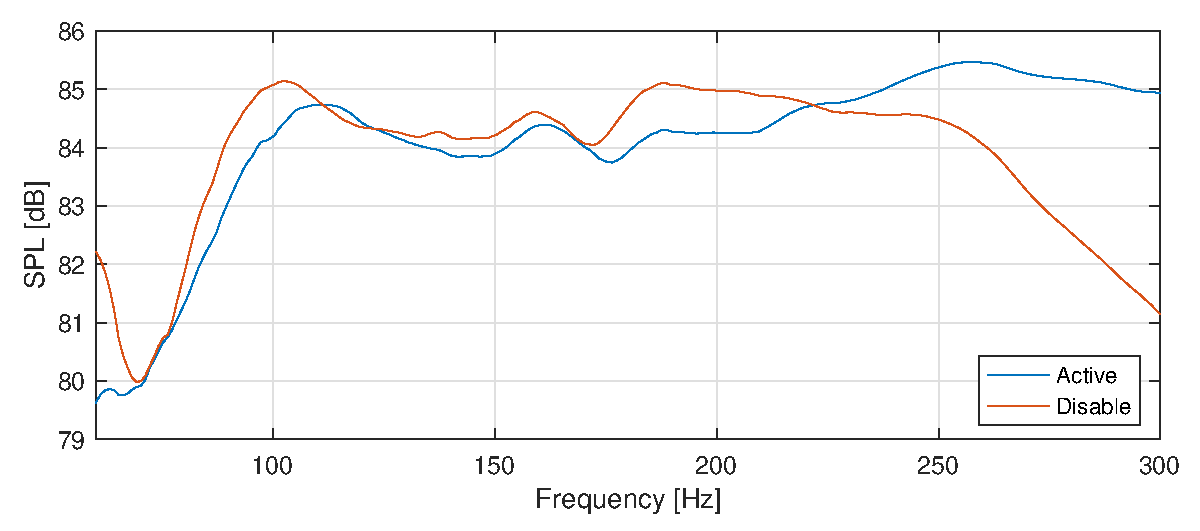
\includegraphics[width=1\textwidth]{beamforming_off_on.eps}
	\caption{The figure shows the \gls{spl} in front for the array with a distance of \SI{4.92}{\meter}, where the blue graph is with beamforming and the red graph is without beamforming}
		\label{fig:beamforming_off_on}
\end{figure}


In \autoref{fig:beamforming_off_on} the graph with and without beamforming shows that the cost filter do have a function and actually works very well from \SI{70}{\hertz} to \SI{250}{\hertz}. Outside those frequency, the graph shows that the array with beamforming does not fit the omnidirectional test. As explain, the cost filter is build on the aligned array en the test is done as a triangle, this might have an effect. To investigate the different between the aligned model and the triangle model with disabled beamforming, the difference in there analytical model will be analysed to research the problem. The following \autoref{fig:beamforming_aligned_triangle} shows the pressure graph of both analytical model in relative to the aligned model.

  \begin{figure}[H]
	\centering
	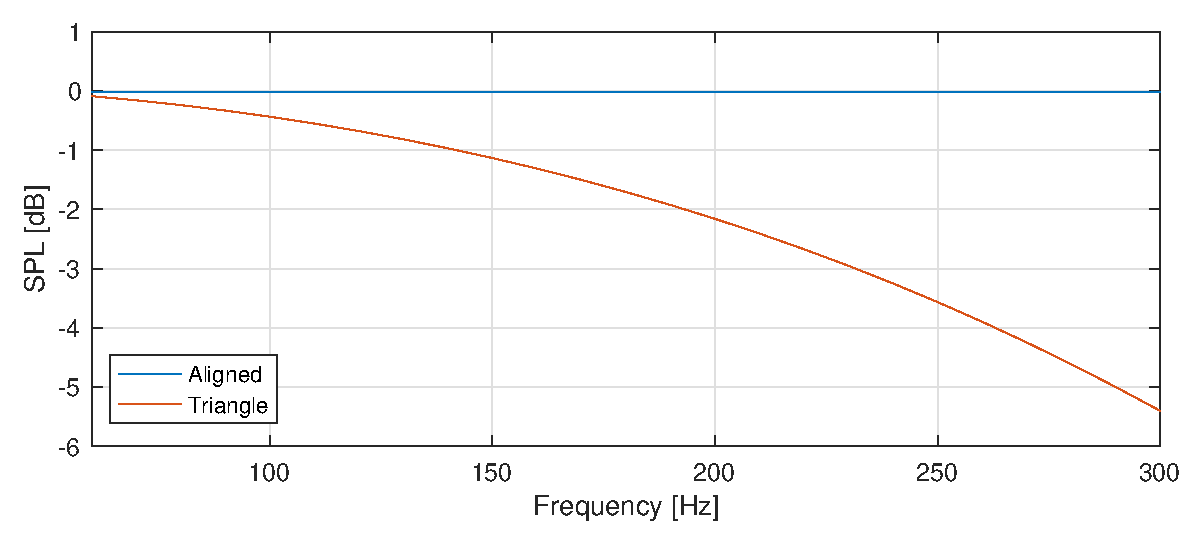
\includegraphics[width=1\textwidth]{beamforming_aligned_triangle.eps}
	\caption{The figure shows the relative pressure in front for the aligned array and the triangle array without beamforming}
		\label{fig:beamforming_aligned_triangle}
\end{figure}

The difference in the analytical models in \autoref{fig:beamforming_aligned_triangle} supports that the pressure between the aligned model and the triangle model without beamforming is different. The triangle model drops in pressure when the frequency go to \SI{30}{\hertz} as in \autoref{fig:beamforming_off_on} but more drastic. This shows that changing from the aligned model to the triangle model that the cost is different specially on the high frequency as also is seen in \autoref{fig:beamforming_off_on}. This model change is then one of the factor that do that the graph with beamforming disabled in \autoref{fig:beamforming_off_on} have a offset in raising frequency. The following \autoref{fig:beamforming_off_on_corrected} shows the graph where the difference from \autoref{fig:beamforming_aligned_triangle} is added to the triangle model without beamforming in  \autoref{fig:beamforming_off_on}

  \begin{figure}[H]
	\centering
	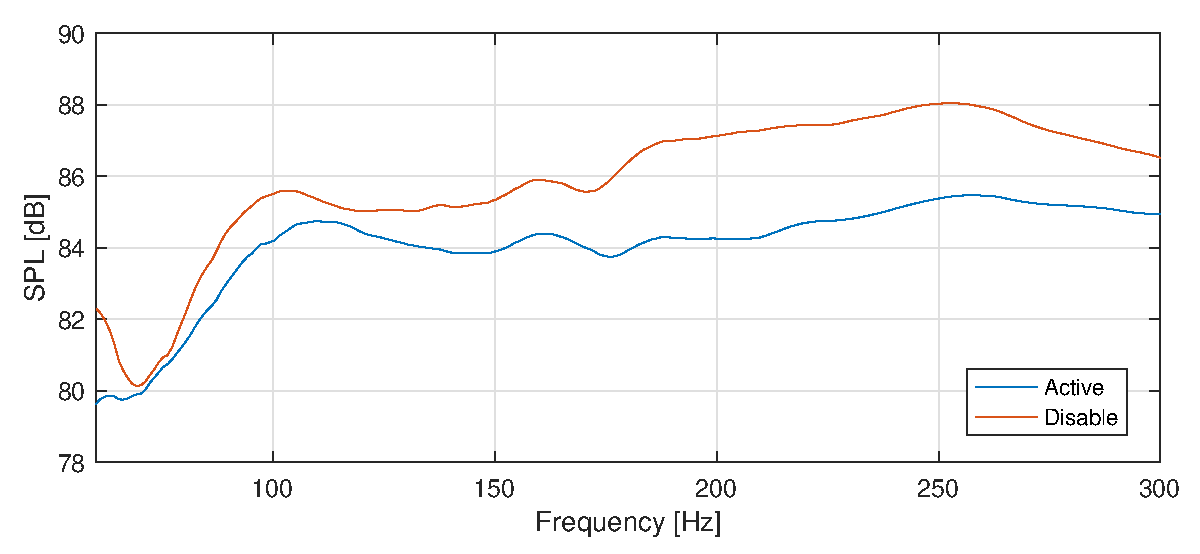
\includegraphics[width=1\textwidth]{beamforming_off_on_corrected.eps}
	\caption{The figure shows the \gls{spl} in front for the array with a distance of \SI{4.92}{\meter}, where the blue graph is with beamforming and the red graph is without beamforming and with the analytical correction}
		\label{fig:beamforming_off_on_corrected}
\end{figure}

At this point, the cost filter seems to fit very well according to the graphs in \autoref{fig:beamforming_off_on_corrected}. It can be seen that there is a gain offset of \SI{2}{\decibel} otherwise both graph do have much similar shape. 

It is interesting to see how the beamforming filter does all around the speaker array. Therefore the different between the array with active and disabled beamforming will present next. The analytical correction is not added to the beamforming polar plot. The following \autoref{fig:polar_plot_dif_result} shows the ploar plot of the difference. 


 \begin{figure}[H]
	\centering
	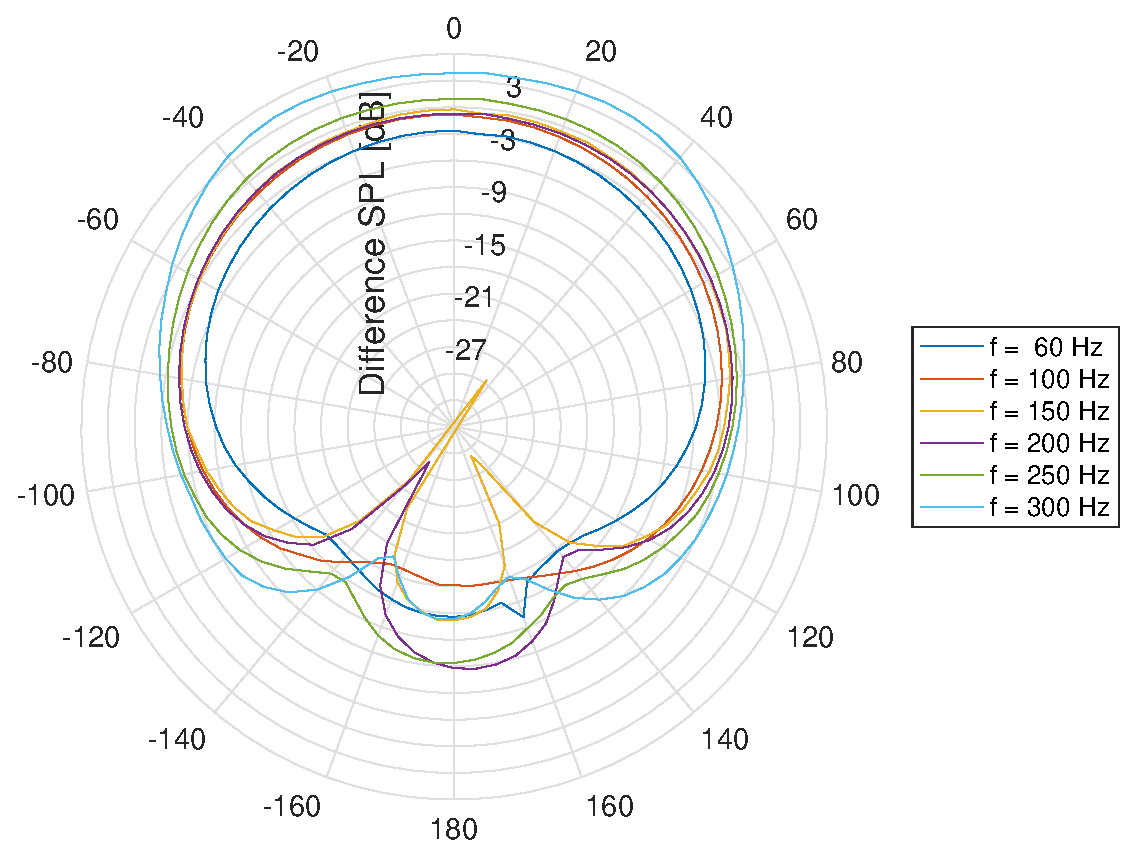
\includegraphics[width=0.9\textwidth]{polar_plot_dif_result.eps}
	\caption{The figure shows a polar plot of the difference \gls{spl} between the array where the beamforming is active and disabled}
		\label{fig:polar_plot_dif_result}
\end{figure}




\section{Conclusion}
It can be concluded that the cost filter works as intended but there is approximate \SI{2}{\decibel} gain differ in the measurement over most of the frequency with beamforming active and with beamforming disabled when the analytical correction is added to the measurement. 


